\newpage
\subsection{Log Messages}
\subsubsection{Ausgangslage}
Log Nachrichten werden beim  starten und stoppen von VPN Tunnels erzeugt und in der Datenbank gespeichert. \\
Dieser Vorgang wird im Frontend gestartet und lösst im Backend einen Thread mit unbekannter Laufzeit aus. Dieser Thread interagiert mit der Vici Schnittstelle und erhält beim Auf-/Abbauen der Verbindungen einen Python Generator als Rückgabewert, welcher bei jeder Iteration ein ordered Dictionary mit Loginformationen enthält. Diese Logs werden nun bei jedem Iterationsschritt in der Datebank persistiert.\\ Dieser Prozess ist an den Verbindungsaufbau des strongSwans gekoppelt und kann daher bis zu mehreren Minuten andauern kann.

\subsubsection{Problematik}
Das Frontend möchte nun jedoch möglichst in Echtzeit an diese Loginformationen kommen und nicht bis auf das Ende der Iterationen warten, sonder die einzelnen Iterationsschrite mitverfolgen.

\subsubsection{Lösungsansatz}
Beim aufruf der Connections Seite wird einen HTTP Long Polling Request ausgelösst, der zuest alle Logs, die älter als 5 Minuten sind, aus der Datenbank löscht und die restlichen dem Frontend zurück gibt. Dies führt dazu, dass ein neuer Request gestartet wird, welcher den neusten Log als Parameter mit gibt und nun nur noch neuere Logs übermittelt werden. Das ganze wird wiederholt, bis die Connections Seite verlassen wird.\\
\begin{figure}[H]
\centering
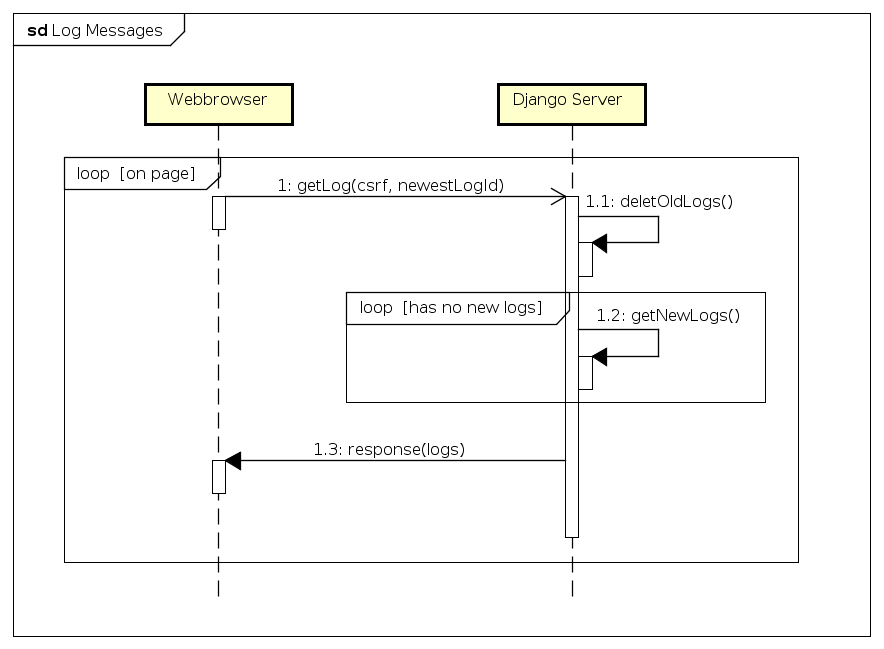
\includegraphics[width=400pt]{images/log_messages_seq.png}
\caption[Log Messages Sequenzdiagramm]{Log Messages Sequenzdiagramm}
\end{figure}